% Chapter Template

\chapter{Theoretical overview} % Main chapter title

\label{Chapter2} % Change X to a consecutive number; for referencing this chapter elsewhere, use \ref{ChapterX}

\lhead{Chapter 2. \emph{Theoretical overview}} % Change X to a consecutive number; this is for the header on each page - perhaps a shortened title

Standard model of elementary particles is a theory emerged in 1960s and 1970s describing all of the known elementary particles and interactions except gravity. The final formulation of Standard model incorporates several theories: quantum electrodynamics, Glashow-Weinberg-Salam theory of electroweak processes and quantum chromodynamics, all of them describing the relations between quarks and fermions. First steps towards formulation of Standard model occurred in 1960. when Sheldon Glashow unified electromagnetic and weak interactions. In 1967. Steven Weinberg and Abdul Salam are using Higgs mechanism in the electroweak theory explaining the origin of mass for elementary particles. After discovery of neutral currents which arise from the exchange of the neutal Z boson, electroweak theory becomes generally accepted. W and Z bosons were discovered in 1981 at CERN, and their masses were in agreement with the Standard model prediction. Theory describing strong interactions got itćs final form in 1974. when it was shown that hadrons are consisting of quarks. There are evidences which show the Standard model is not a final theory of elementary particles, but so far it's predictions were confirmed every time through numerous experimental tests. Standard model has one additional nice property, all fundamental interactions arise from one general principle, the requirement of local gauge invariance. \\
In this chapter a brief overview of the standard model particles and interactions will be shown with the emphasis on the W boson and b quarks which are the most relevant for this thesis. Cross section determination at hadron colliders will be shown.  In the last part of the chapter historical account of the development of W+b-jets theoretical calculations is described together with the existing experimental results.

%----------------------------------------------------------------------------------------
%	SECTION 1
%----------------------------------------------------------------------------------------

\section{Standard model overview}

\par Elementary particle physics is described within a framework of standard model. We usually imagine particles as point like objects and some forces between them. Particles, or matter, are fermions, leptons of quarks of spin $s=1/2$. There are three charged leptons, electron, muon and tau which properties are the same except for their mass. Each of the leptons has a corresponding neutrally charged neutrino which has a very small mass. There are six different types of quarks with charge either $Q=2/3$ of $Q=-1/3$. They also carry one additional quantum number which is color charge. All objects observed in nature are colorless giving raise to the concept of quark confinement. Colorless composite objects are classifies into two categories. Bayons are fermions which are made out of three  quarks, for example proton or neutron. The other category are mesons which are made of two quarks like pions. Matter is divided into three categories which are identical except for the masses of the particles. 
\par From the point of view of the quantum field theory, standard model is based on a gauge symmetry $SU(3)_C \times SU(2)_L \times U(1)_Y$. Strong interaction is described by $SU(3)_C$, while electroweak sector is described by $SU(2)_L \times U(1)_Y$. All interactions within Standard Model are mediated by an elementary particle which is a spin 1 boson. In the case of electromagnetic interaction, mediator is massless photon thus the range of electromagnetic interaction is infinite. For weak force mediators are three massive bosons $W^{\pm}$ and $Z$ and it's range is very small ($10^{-16}$). These four bosons are the gauge bosons of $SU(2)_L \times U(1)_Y$ group. The interaction between electroweak bosons is allowed in the Standard Model in a way that charge conservation principle remains valid. Strong force is mediated by the exchange of 8 massless gluons which are gauge bosons for $SU(3)_C$. Although gluons are massless, the range of the strong force is not infinite. Because of the effect of confinement, the range of the strong force is approximately the size of the lightest hadrons ($10^-{13} cm$). 
\begin{figure}[htbp]
	\centering
		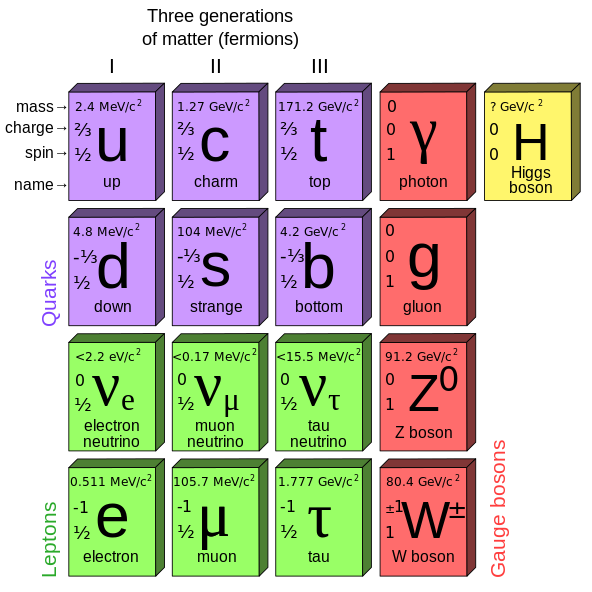
\includegraphics[width=0.5\textwidth]{Figures/Elementary_Particles.png}
		%\rule{35em}{0.5pt}
	\caption[List of Standard model elementary particles]{List of Standard model elementary particles.}
	\label{fig:SM_particles}
\end{figure} 
\par Scalar sector of the standard model has been experimentally confirmed only recently \cite{Aad:2012tfa,Chatrchyan:2012ufa}. The fact that weak gauge bosons are massive indicates that $SU(2)_L \times U(1)_Y$ is not a good symmetry of the vacuum. In contrast with photon being massless, $U(1)_em$ is a good symmetry of the vacuum which means that $SU(2)_L \times U(1)_Y$ electroweak symmetry is somehow spontaneously broken to $U(1)_em$ of electromagnetism. Spontaneous symmetry breaking is implemented through Higgs mechanism which gives masses to $W\pm$ and $Z$ boson, fermions and leaves photon massless. The details of the mechanism can be found elsewhere \cite{Griffiths:1987tj} but the main point is that the mechanism also predicts a new scalar and electrically neutral particle which is called Higgs boson. The search for Higgs boson lasted few decades before finally in 2012, a new particle was discovered with mass of 125 GeV. In subsequent years, properties of this new particle have been measured and at this point, all measurements agree with Standard Model predictions for Higgs boson.    
   

%-----------------------------------
%	SUBSECTION 1.1
%-----------------------------------

\subsection{Bottom quarks}

Bottom quark was first predicted by Makoto Kobayashi and Toshihide Maskawa in 1974 when extending Cabbibo weak mixing angle to take into account CP violation observed in neutral K mesons. \cite{Kobayashi:1973fv} The name "bottom" was introduced in 1975 by Haim Harari. The bottom quark was discovered in 1977 by the Fermilab E288 experiment team led by Leon M. Lederman through the observation of $\Upsilon$ resonance. \cite{PhysRevLett.39.252} Kobayashi and Maskawa won the 2008 Nobel Prize in Physics for their explanation of CP-violation. 
\par At the the LHC, the main production mechanism for b quarks is through strong interaction ($g\rightarrow bb$) and top quark decay ($t\rightarrow Wb$). Every b quark, after production, goes through the process of hadronisation, forming one of the color neutral B mesons. B meson decays electromagnetically if produced in excited state to the ground state. Lowest state B mesons decay weakly, resulting in relatively long lifetime of 1.5 ps. According to CKM matrix \ref{eq:ckmmatrix}, b quark can decay either to c quark ($\approx 95\%$ of the cases) or u quark ($\approx 95\%$ of the cases). Long lifetime of b quark makes it possible to traverse a substantial distance inside the detector. This fact is used in the creation of various b-tagging algorithms which are taking into account tracks originating from displaced verices, discussed in Section 
\ref{Chapter4}.

\begin{equation} 
\begin{pmatrix}
V_{ud} & V_{us} & V_{ub} \\
V_{cd} & V_{cs} & V_{cb} \\
V_{td} & V_{ts} & V_{tb} 
\end{pmatrix} 
= \begin{pmatrix}
0.974 & 0.225 & 0.003 \\
0.225 & 0.973 & 0.041 \\
0.009 & 0.040 & 0.999 
\end{pmatrix} 
\label{eq:ckmmatrix} 
\end{equation}


%-----------------------------------
%	SUBSECTION 1.2
%-----------------------------------

\subsection{Discovery and role of W boson}

W boson is one of the massive mediators of weak interaction with a mass of $m_W=80.1$ GeV.
The theory of the weak interactions got it's final form in 1968 when Sheldon Glashow, Steven Weinberg, and Abdus Salam unified a theory of electromagnetism and weak interactions. The discovery of W and Z bosons at UA1 and UA2 experiments was one of the major successes of the CERN experimental facility. Super Proton Synchrotron was the first accelerator powerful enough to produce W and Z bosons. Both collaborations reported their findings in 1983 \cite{Arnison:1983rp,Banner:1983jy}.
W boson at the LHC is primarily produced through quark-antiquark annihilation. In majority of the cases, W boson decays to quark-antiquark pair ($66\%$). Other decay channels include creation a lepton and it's corresponding neutrino($\approx 10\%$ per lepton generation). This decay channel was the most important for W boson discovery and it's still essential for W boson detection at hadron colliders despite the large hadronic backgrounds. 
\par Study of W+jets production at hadron colliders started in 1980s motivated by the top quark searches. Additional jets either come from radiation of additional quarks or gluons. However, because they carry color charge, quarks and gluons undergo the process of parton shower and hadronization forming jets in the detector. Parton shower is the process in which a high energy colored particle emits a low energy colored particle while hadronization is the process in which colored particle combine to form color neutral particles. Parton shower and hadronization cannot be computed analytically, but have to be modeled using Monte Carlo simulations. As a result of these processes, in the final state there can be a number of jets that doesn't  correspond to the number of incoming partons. This becomes relevant when trying to form an inclusive W+jets sample from exclusive (W + 1 jet, W + 2 jets...) samples and some process of matching has to be performed in order to avoid double counting. Matching procedure is described in detail in \cite{Campbell:2008cr}.  
\par Many theoretical issues arise when trying to compute cross sections for W+jets processes. Divergences while calculating amplitudes come from emission of soft particles or collinear jets. These problems are solved by introducing a cut-off called factorization scale. Other divergences come from integrating higher-order loops. Usually this type of divergence is than included into renormalized coupling constant. This procedure, however introduces a certain scale dependence into the result which will be discussed further in Section \ref{subsec:2.1}. 


%----------------------------------------------------------------------------------------
%	SECTION 2
%----------------------------------------------------------------------------------------

\section{W + b jets at hadron colliders}

First theoretical computations of W boson in association with b jets were published in 1993 \cite{Mangano:1992kp}, however only recently enough luminosity has been collected at hadron colliders to be able to make cross section measurements. This process was first interesting as a background to top quark searches and measurements where top quark decays to W boson and a b quark. In past few years, with the Higgs boson discovery, an important open question is whether the new particle also couples to fermions, and in particular to bottom quarks. Determination of this coupling requires
direct measurement of the corresponding Higgs boson decay, as recently reported
by the CMS experiment in the study of Higgs decays to bottom quarks \cite{Chatrchyan:2013zna,Chatrchyan:2014vua}.
Standard model Higgs boson branching ratio for decays into a bottom quark-antiquark
pair (bb) is $\approx 58\%$. Study of this decay channel is therefore essential in determining the nature of the newly discovered boson. The measurement of the H $\rightarrow$ bb decay will be the first direct test of whether the observed boson interacts as expected with the quark sector, as the coupling to the top quark has only been tested through loop effects. However, the large backgrounds for this measurement make it essential that all the contributing processes including W+b jets are well understood.
There are also Beyond Standard Model searches where contributions from this process is substantial including some Supersymmetry searches with lepton, b jets and missing energy in the final state.

Soft and collinear divergences are naturally avoided in processes with b jets because of relatively high mass of b quark which means that the scale of the process doesn't go below $2m_b$.


%-----------------------------------
%	SUBSECTION 2.1
%-----------------------------------

\subsection{Cross sections at hadron colliders}
\label{subsec:2.1}

	Determining cross sections for processes at hadron collides is not an easy task. With proton being a composite object consisting of partons, it is necessary to include it's internal structure as well as the diagrams for hard scattering of interest. This means soft and hard processes are occurring in the same event. Quarks and gluons within proton interact through strong force and are described using quantum chromodynamics. Two processes make it possible to perform calculations within the QCD, asymptotic freedom and factorization theorem. Since strong force coupling constant $\alpha_s$ depends on the scale, for high momentum transfers ($Q >> \Lambda_{QCD}\approx 200$MeV) it becomes sufficiently small to make perturbative expansion in $\alpha_s$ possible. This feature is called asymptotic freedom and it is used to determine the hard process cross section. Figure \ref{fig:alpha_s} shows the results of the $\alpha_s$ measurements which is in complete agreement with the QCD predictions of asymptotic freedom. \\
\begin{figure}[htbp]
	\centering
		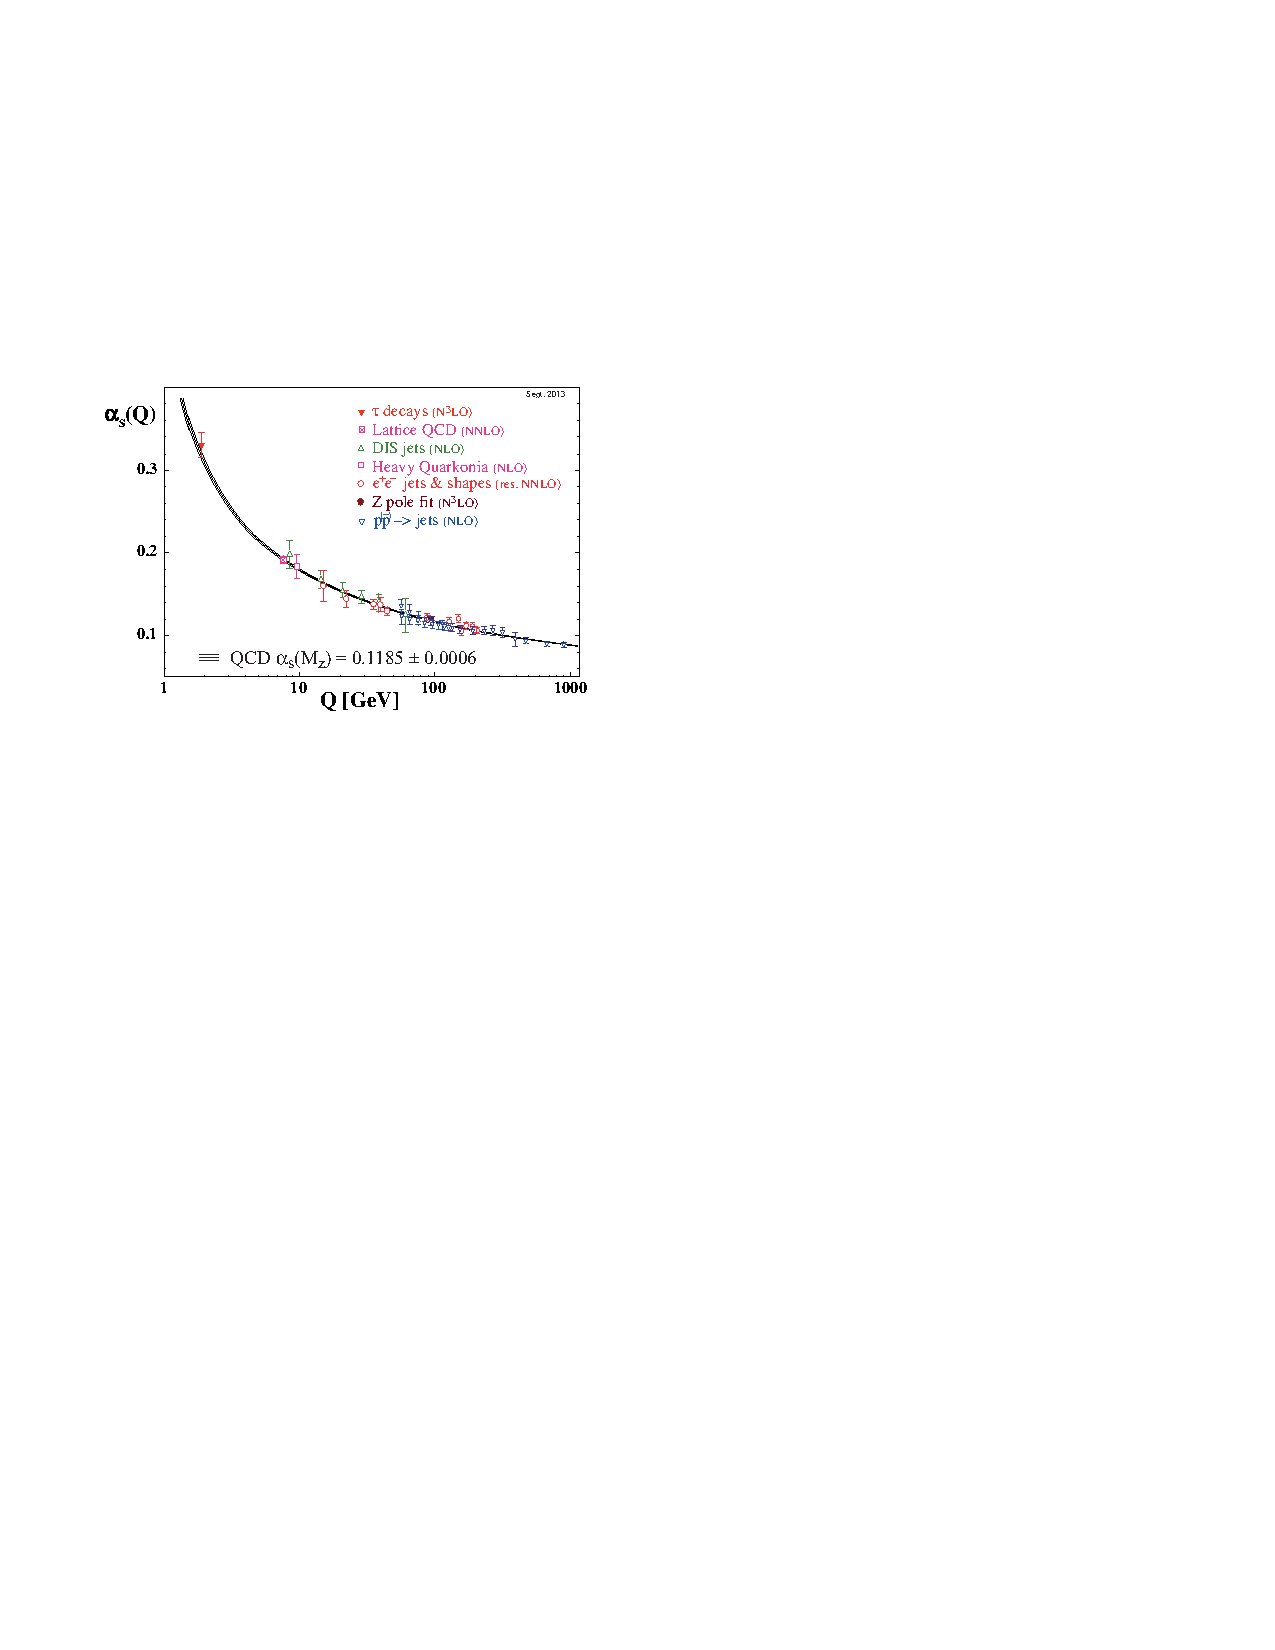
\includegraphics{Figures/alpha_s.pdf}
		%\rule{35em}{0.5pt}
	\caption[Strong force coupling constant]{Summary of measurement of strong coupling constant $\alpha_s$ \cite{Agashe:2014kda} }
	\label{fig:alpha_s}
\end{figure}

	\par Perturbative QCD cannot be used if the momentum transfer values are small and the coupling constant becomes large. This phenomenon is called \textit{confinement} and it requires different treatment for the quarks inside the proton. Internal structure of a proton is described using parton distribution functions which  are determined through deep inelastic scattering experiments. Parton distribution functions for each of the partons inside a proton is shown in Figure \ref{fig:MSTW} made with one specific PDF function(MSTW). Using DGLAP equations, it is possible to evolve the PDFs for any momentum transfer value which is described in detail in \cite{Campbell:2006wx} 

\begin{figure}[htbp]
	\centering
		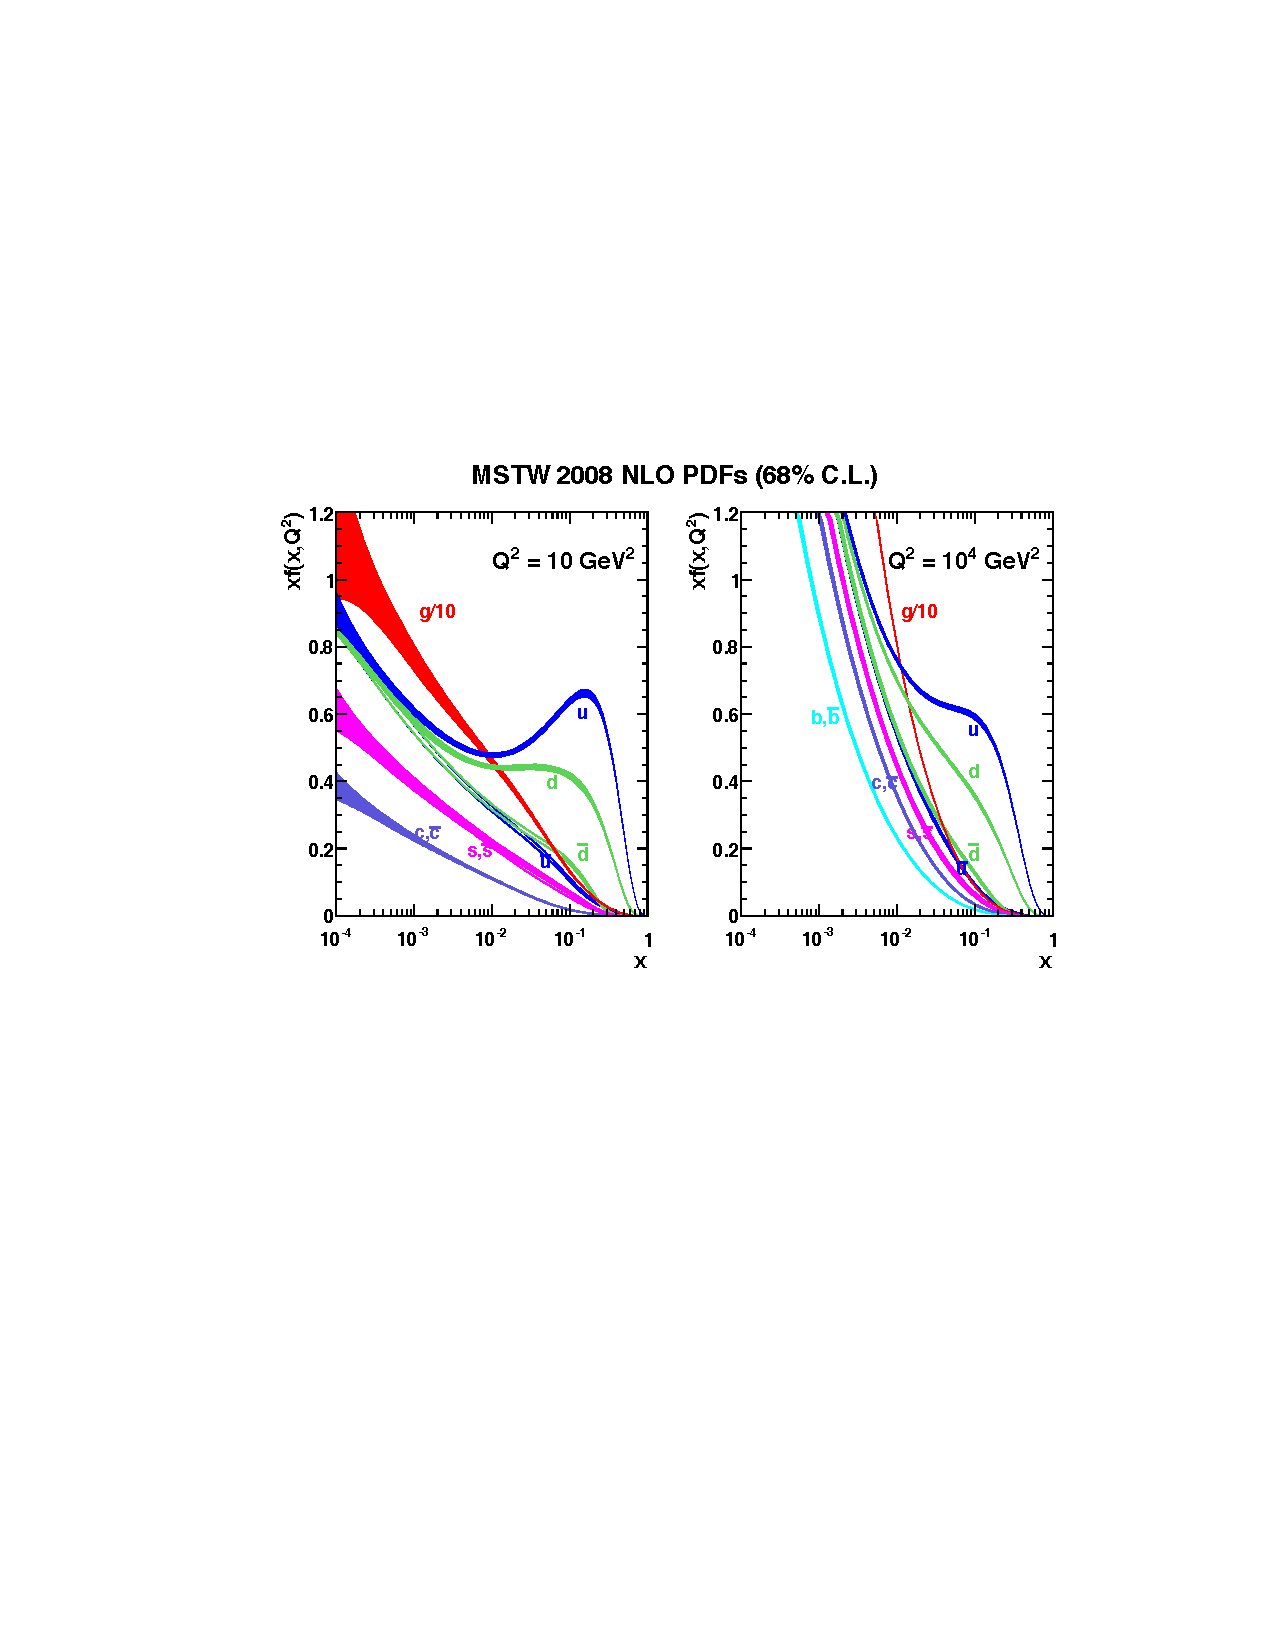
\includegraphics{Figures/MSTW.pdf}
		%\rule{35em}{0.5pt}
	\caption[Parton distribution functions for different momentum transfers]{Parton distribution functions calculated by the MSTW group for $Q=10$GeV and $Q=10^4$GeV \citep{Martin:2009iq}}
	\label{fig:MSTW}
\end{figure}

While performing perturbative QCD calculations, it is important to impose conditions to the final state in order to avoid soft and collinear divergences. Collinear divergences originate from configurations with a small opening angle between jets. Soft divergences appear when quark or gluon is irradiated at low momentum. Factorization scale is introduced as a cut-off for diagram calculation below which perturbative QCD calculation is not performed which means that hard scattering between partons is independent from the parton internal structure. The main point of the factorization theorem  is that because of energy dependence of strong coupling constant, hard and soft part of the process are happening at different time scales ans soft part is factorized inside a parton distribution function.
\begin{figure}[htbp]
	\centering
		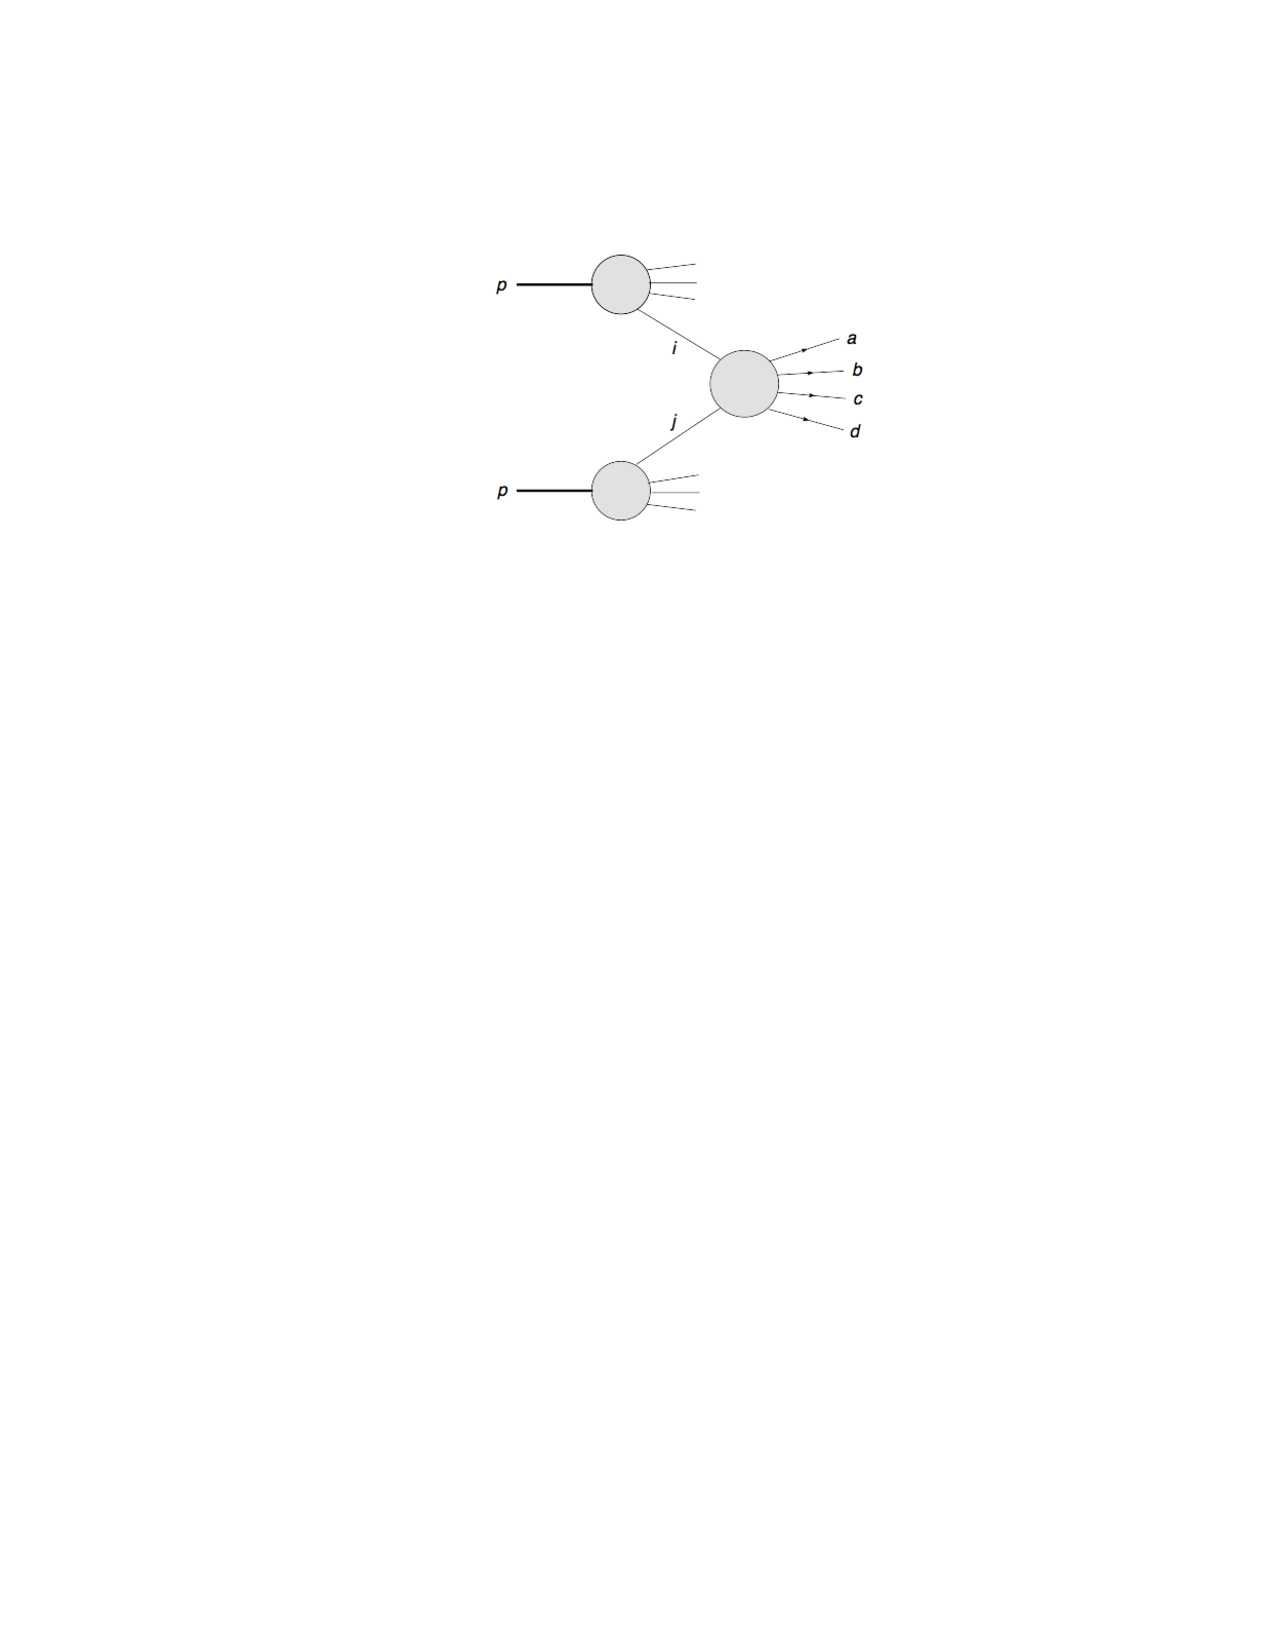
\includegraphics{Figures/diagram.pdf}
		%\rule{35em}{0.5pt}
	\caption[Drawing of a proton-proton collision]{Drawing of a proton-proton collision.}
	\label{fig:pp_drawing}
\end{figure}
Drawing of a proton proton collision is shown in figure \ref{fig:pp_drawing}. If we want to calculate the cross section for some process where there are two protons in the initial state and some interesting final state which we call X, according to \cite{Campbell:2006wx}, necessary steps are:
\begin{enumerate}
	\item Identify the leading order partonic processes that contribute to X
	\item Calculate the corresponding hard scattering cross section
	\item Determine the appropriate PDFs for initial state partons
	\item Make a specific choices for factorization($\mu_F$) and renormalization($\mu_R$) scales
	\item Perform integration over the fraction of momentum available for a given parton(x)  
\end{enumerate}
The cross section at hadron collides is thus a convolution of the hard scattering perturbative cross section and two incoming parton distribution functions.
\begin{equation}
\sigma_{AB} = \sum\limits_{n=1}^{\infty} \alpha_{s}^{n}(\mu_{R}^2)\sum\limits_{i,j} \int dx_1 dx_2 f_{i/A}(x_1,\mu_{F}^2) f_{j/B}(x_2,\mu_{F}^2) \sigma_{ij \rightarrow X}^{(n)}(x_1 x_2s,\mu_{R}^2,\mu_{F}^2)
 \label{eq:xsec}
\end{equation} 
\par Equation \ref{eq:xsec} shows cross section perturbation series in $\alpha_s$, $n$ denotes the order of the series where $n=1$ is leading order, $n=2$ is next to leading order, etc. 
Hard process cross section between two partons $\sigma_{ij \rightarrow X}^{(n)}$ is computed in the framework of perturbative QCD and depends on $s$ which is squared center of mass energy. Two parton distribution functions are denoted with $f_{i/A}$ and $f_{j/B}$ and correspond to the probability density that parton $i$($j$) with proton momentum fraction $x_1$($x_2$) will be found inside a proton. Sum over all combinations of partons has to be computed. Integral over available phase space for proton fraction momentum $dx$ is usually carried out by simulations.\\ 
Here $\mu_F$ represents \textit{factorization scale} and $\mu_R$ is \textit{renormalization scale} for running coupling constant. They are arbitrary cut-offs used to remove nonperturbative effects and be able to make perturbative calculations. If cross section is computed in full series, $\mu_F$ and $\mu_R$ should cancel out, and scale dependence should disappear. However, since fewer orders are used and some residual scale dependence is still present. This dependency can be used to estimate the contribution of the missing orders in the series.  
\par Usually factorization and renormalization scales are chosen to be identical and close to the scale of the process in question. 

\textbf{NAPISATI PRIRODNE IZBORE SKALE!!!}  

\begin{figure}[htbp]
	\centering
		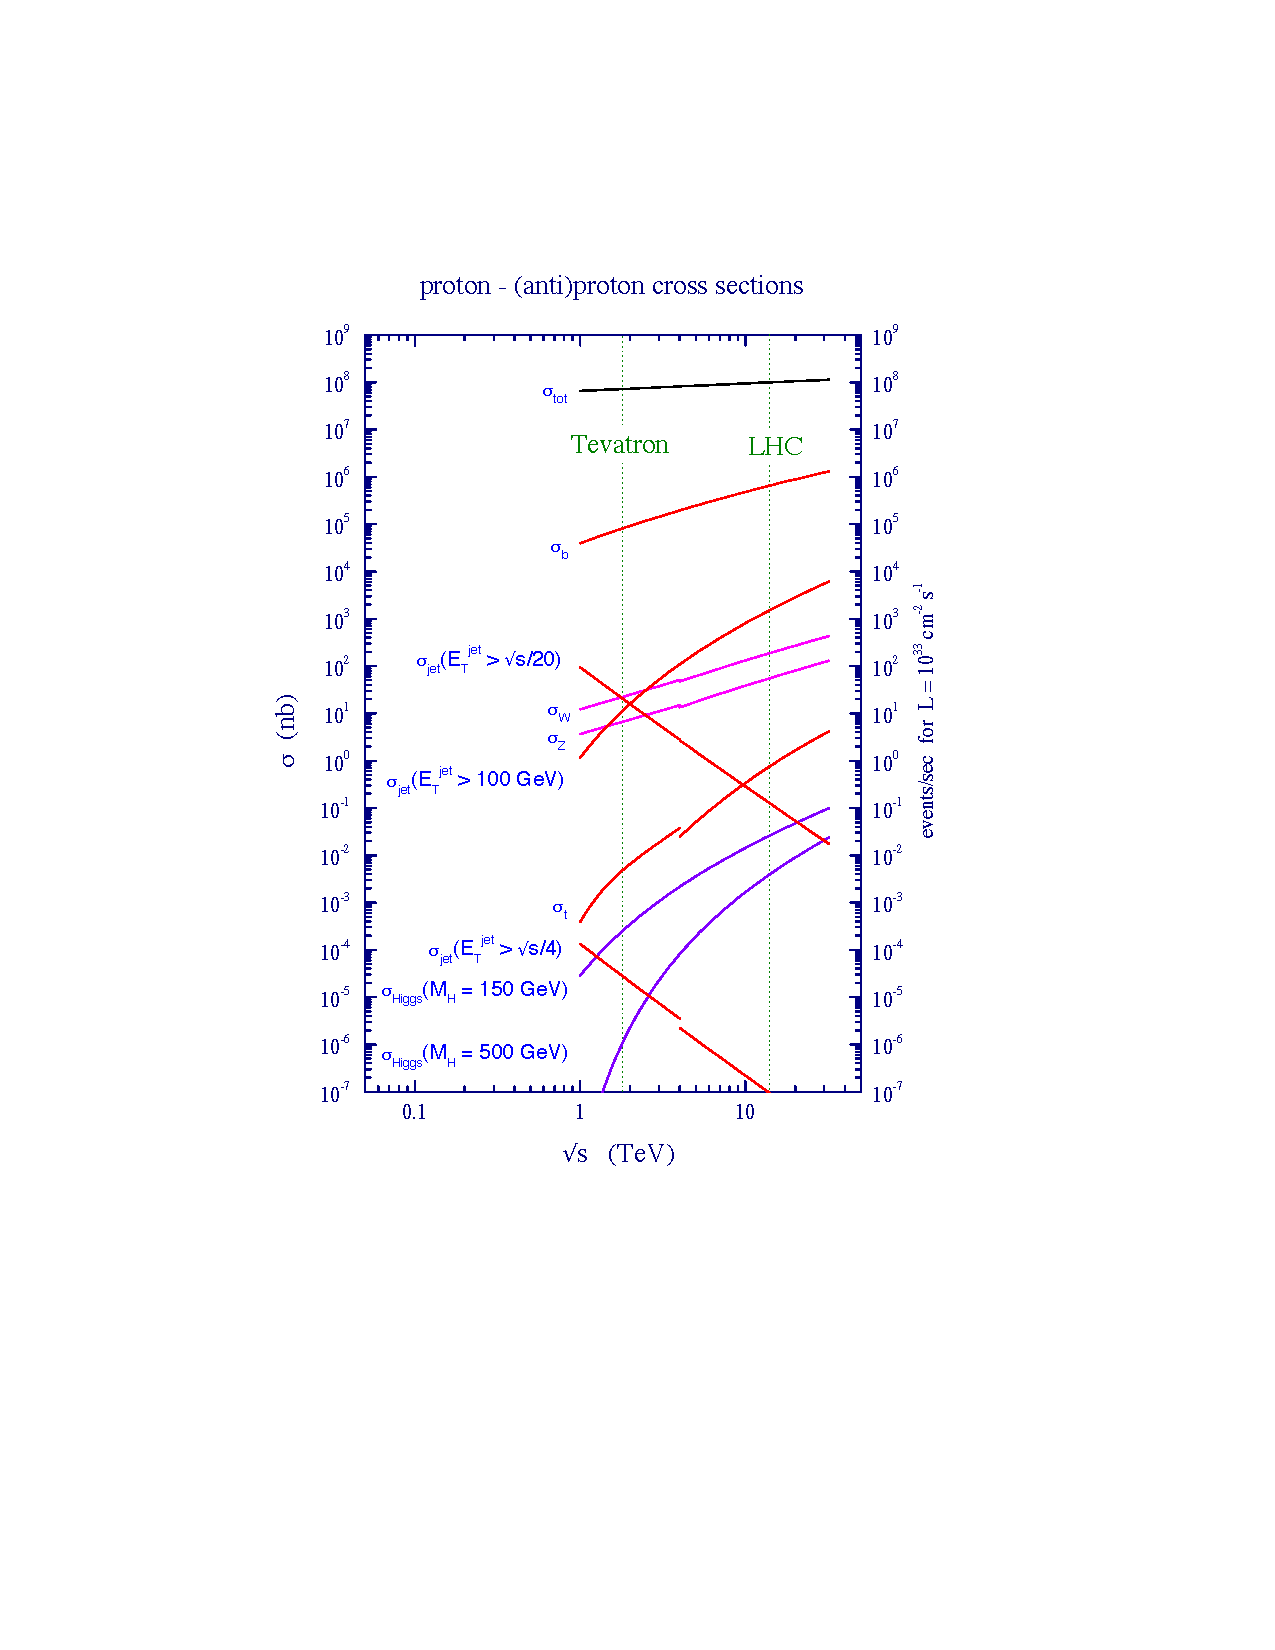
\includegraphics{Figures/pp_xsec.pdf}
		%\rule{35em}{0.5pt}
	\caption[Proton-proton cross sections]{Standard model cross sections as a function of center of mass energy.\cite{Campbell:2006wx} }
	\label{fig:pp_xsec}
\end{figure}
\par Figure \ref{fig:pp_xsec} shows some interesting Standard model cross sections in proton-proton and proton-antiproton collisions as a function of a center of mass energy. All cross sections have been computed to the NLO order using the above described procedure.

 
%-----------------------------------
%	SUBSECTION 2.2
%-----------------------------------

\subsection{Contributions to Wbb cross section}


From theoretical point of view, calculations of W+b jets processes can be divided into two categories: only light quarks in the initial state shown in figure \ref{fig:LO_diag} (four flavour scheme - 4FS) and b quark in the initial state, usually called five flavor scheme (5FS) shown in Figure \ref{fig:5FS_diag}. Additional contribution to Wbb production at hadron colliders comes from double parton interactions where a W boson and a pair of b quarks is produced in different hard process inside the same collision as shown in Figure \ref{fig:DPS_diag}. This contribution will be discussed in Section \ref{sec:DPS}.

\par The rationale behind using 4FS or 5FS is discussed in detail in \cite{Maltoni:2012pa}. Four flavor scheme approach assumes that bottom quarks are heavy and can only be created as pairs in collisions with high momentum transfer or as a decay product of t quark. Heavy quarks are not included in the initial state and their parton distribution function is set to zero which means an effective theory is created where heavy quarks do not enter the computation of running coupling and the evolution of PDFs. In this approach, it is assumed that scale is of the same order as the other hard scales in the process. If it happens that the scale of the process if much higher than the mass of the b quark, for example in the production of massive bosons, large logarithms of the type $log(Q^2/m_b^2)$ appear and can spoil the convergence of a fixed order perturbative expansion and it introduces large scale dependence into the final result. In five flavor schemes calculations include b quark in the initial state which means some new and simpler processes become available. These calculation allow ressumation of possibly large logarithms of type $log(Q^2/m_b^2)$ into the b quark parton distributions function possibly transforming some higher order calculations into much simpler leading order calculations.  
Their results show that at the LHC 4-flavor calculations are well behaved and two schemes are in good agreement. The typical size of the possibly problematic logarithms in four flavor scheme in hadron colliders is not large enough to spoil convergence. On the other hand, five flavor scheme is less dependant on the scale of the process and show smaller uncertainties which is in general very good for predictions of inclusive observables.  

\par First leading order calculations for associated production of a W boson and heavy quarks at hadron colliders were presented in 1993. Feynmann diagram for leading order W + 2 b jets production is shown in Figure \ref{fig:LO_diag}. Exact leading order matrix element has been computed and higher order corrections were estimated using Monte Carlo. Their results are summarized in the Figure \ref{fig:scale_dep} where the differential cross section for W+2 b jets as a function of a leading b jet $p_T$ is shown. Two scale choices have been studied, first one with $\mu_0=Mbb$ which is the invariant mass of the dijet system and is represented with solid line. Second choice is $\mu_0=m_W+p_T^W$ and is represented with the dotted line. Looking at the normalizations of two diagrams, the difference is clearly visible which indicates a strong total cross section scale dependence. However, the shape of the differential cross section shows the same behavior in both cases which means that the scale only affects total cross section.      
\begin{figure}[htbp]
	\centering
		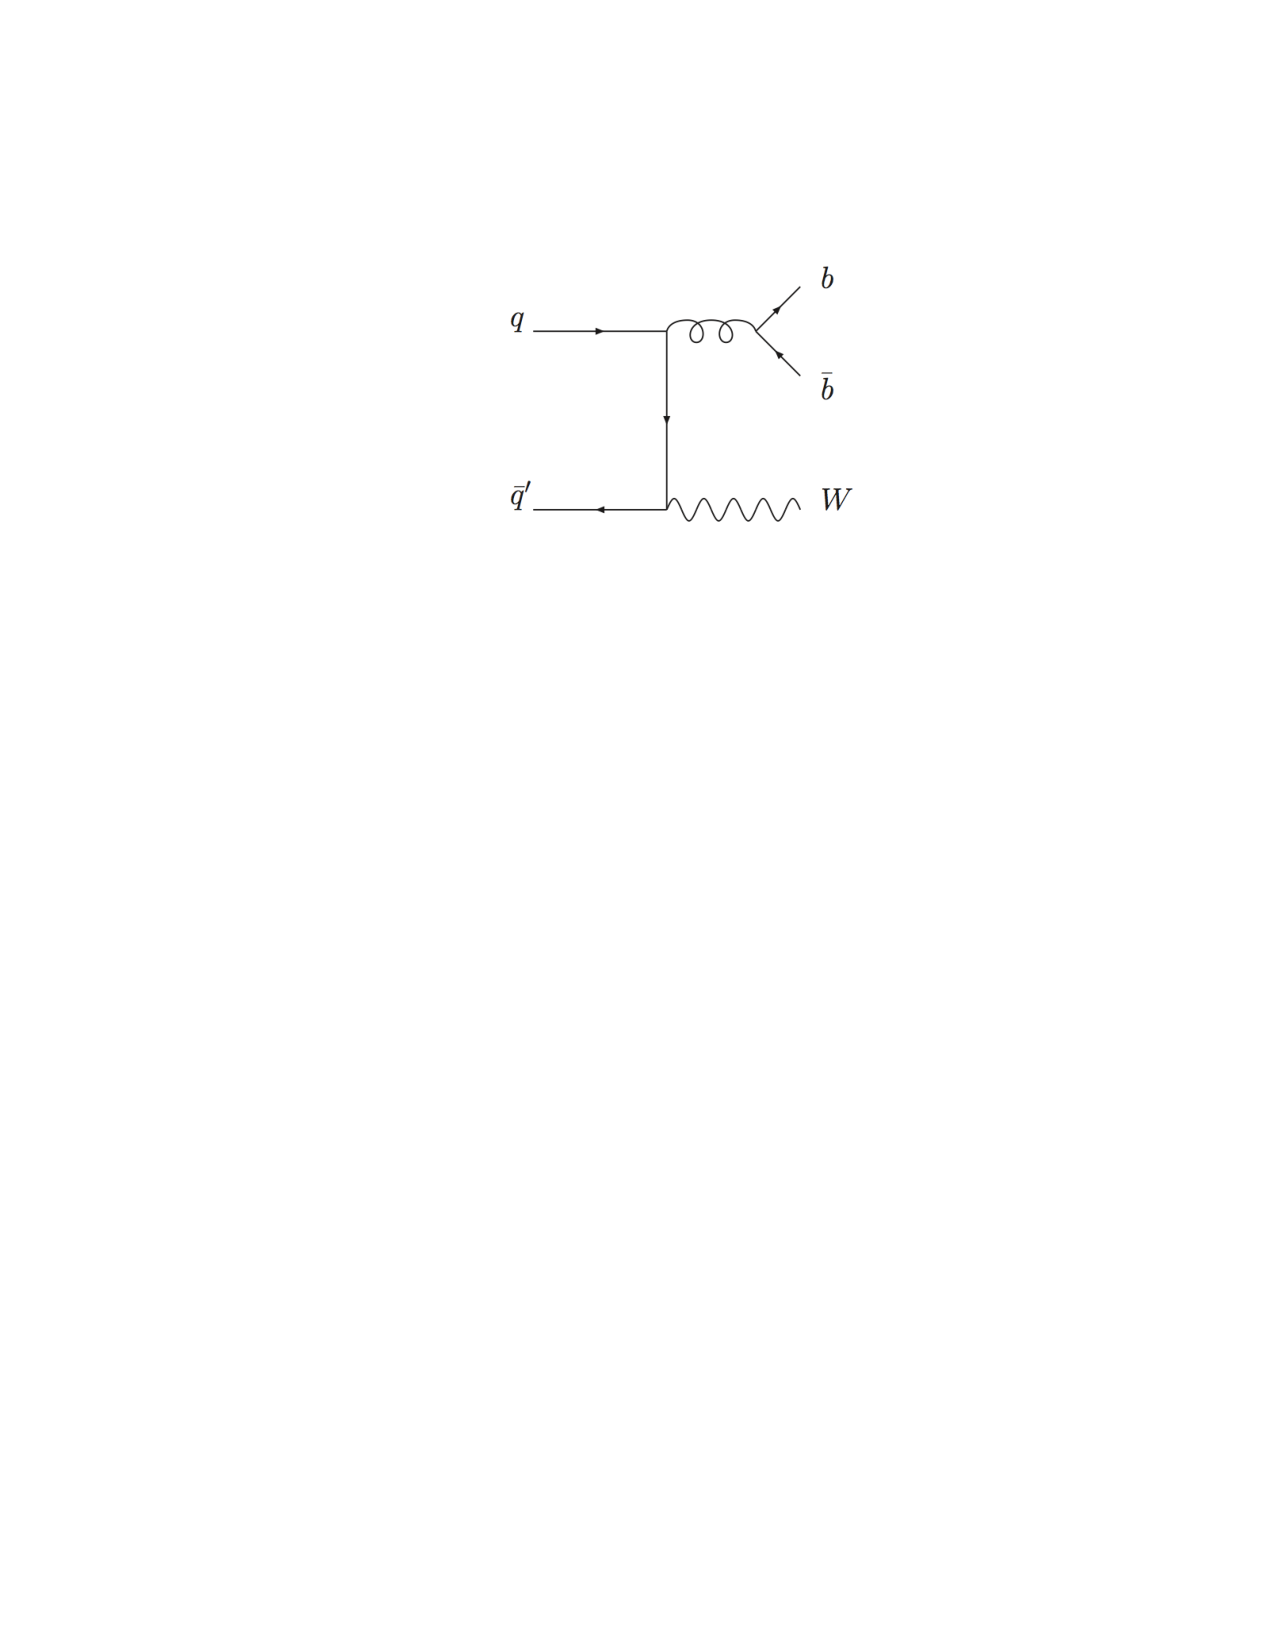
\includegraphics{Figures/LO_diag.pdf}
		%\rule{35em}{0.5pt}
	\caption[Leading order Wbb Feynmann diagram]{Leading order Wbb Feynmann diagram}
	\label{fig:LO_diag}
\end{figure}
\begin{figure}[htbp]
	\centering
		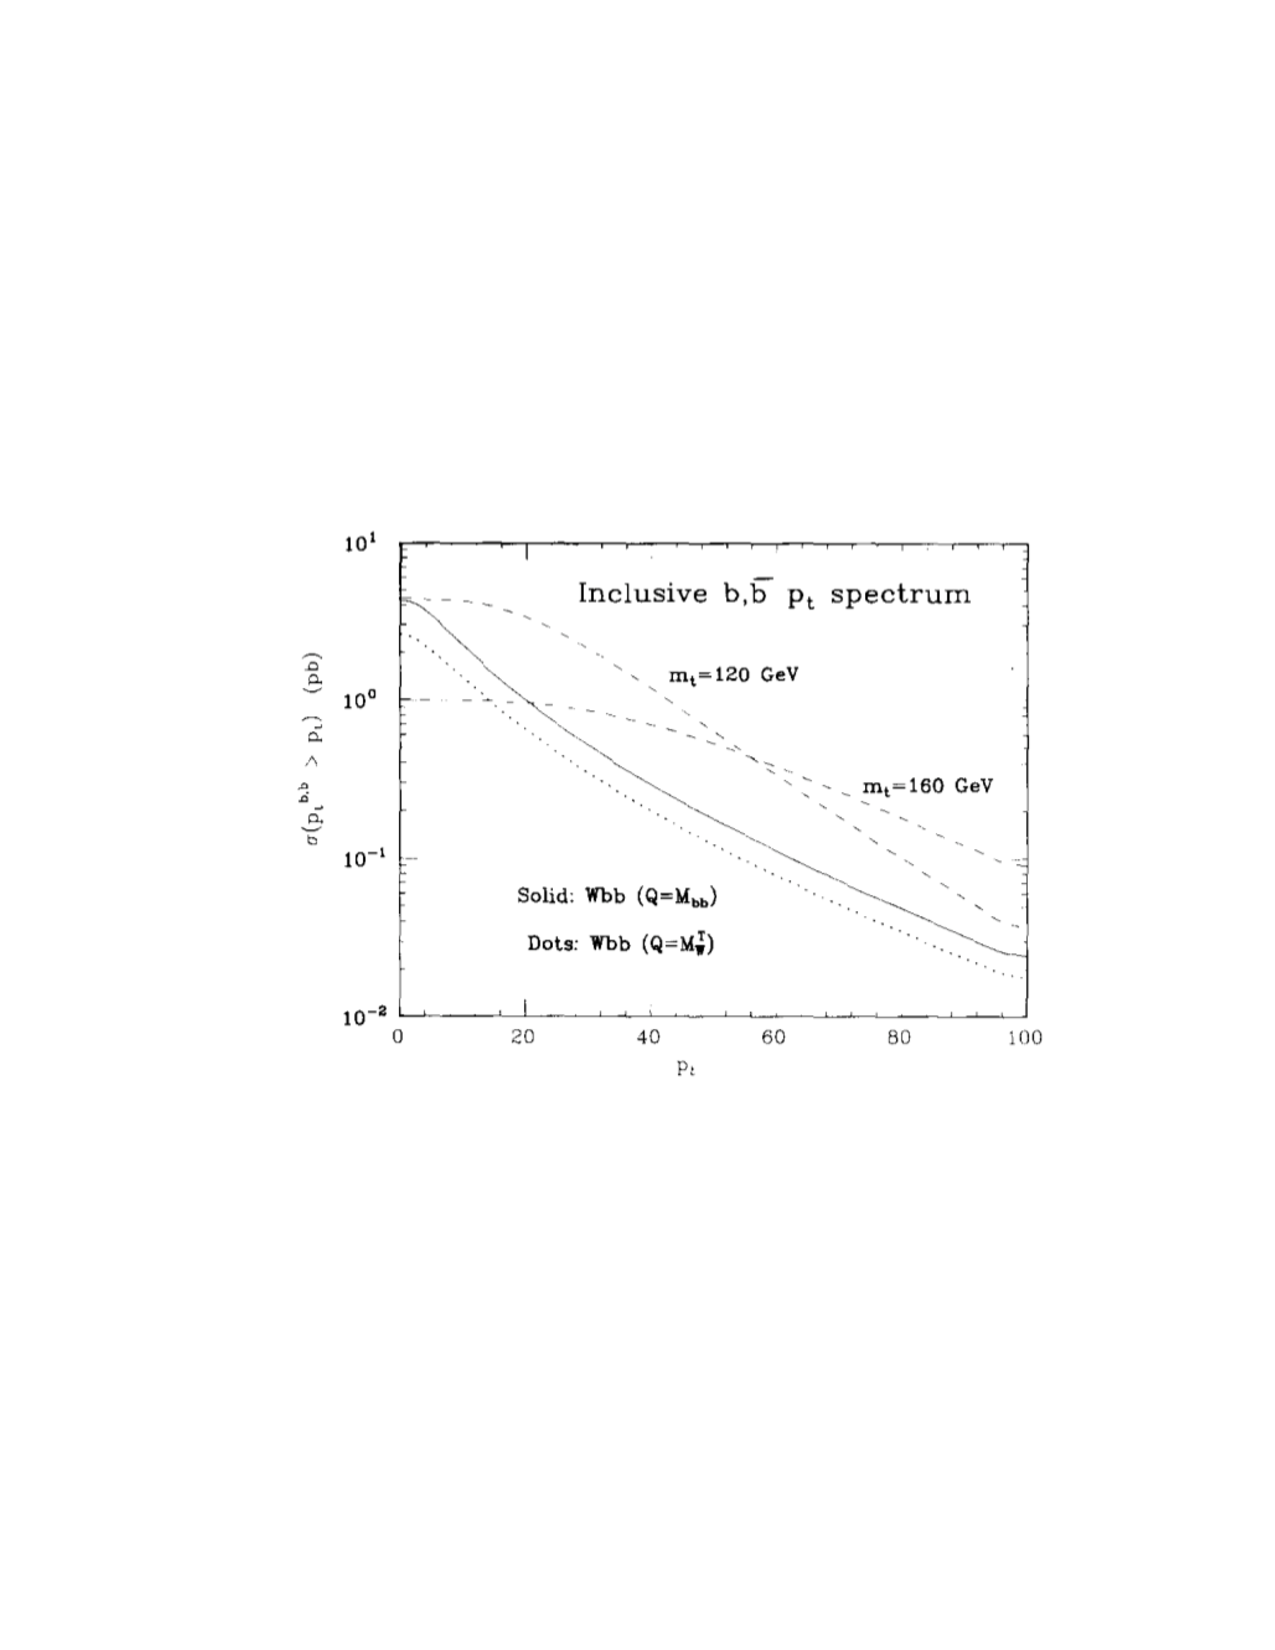
\includegraphics{Figures/scale_dep.pdf}
		%\rule{35em}{0.5pt}
	\caption[Scale dependence of Wbb cross section]{Scale dependence of Wbb cross section}
	\label{fig:scale_dep}
\end{figure}
\par Later development of theoretical calculations was strongly motivated by reducing the scale dependence of the result and it included adding additional partons to the final state. This was a first step towards the full NLO calculation. The only thing missing was taking into account the loop effects. This approach made it possible to access some previously inaccessible kinematics, however at the expense of introducing additional scale dependence. The list of new final states is simple and it includes $Wbbq$, $Wbbq\bar{q}$, $Wbb\bar{q}q'\bar{q'}$... For the measurements at the LHC in particular, calculations for new initial states $qg$ and $gg$ were of great importance. First results for W+2 jets were published in \cite{Ellis:1998fv}. Additional calculations were shown in \cite{Mangano:2001xp} for up to six additional jets in the final state. Although these processes are suppressed by an additional $\alpha_s$ factor, the gluon PDF inside a proton is much larger than anti-quark, so this production mechanism is significant at the LHC energies. 
\par First full NLO calculations were published in 2006\cite{FebresCordero:2006sj}. 
Events with b jet pair in the final state were selected, with of the dijet system $p_T>$15 GeV  and a pseudorapidity less than 2. The results were shown for two categories, inclusive and exclusive, depending on the treatment of extra jets. In the inclusive case events with additional jets were included, while in the exclusive case exactly two jets were required.
Figure \ref{fig:2006_scale} shows the overall scale dependence of LO, NLO inclusive and NLO exclusive total cross-ections, when both renormalization scale and factorization scale are varied independently between $\mu 0/2$ and $4\mu 0$ (with $\mu 0 = m_b + M_W /2)$, including full bottom-quark mass effects. NLO cross sections have a reduced scale dependence over most of the range of scales shown, and the exclusive NLO cross-section is more stable than the inclusive one especially at low scales.
This is consistent with the fact that the inclusive NLO cross-section integrates over the
entire phase space of the $qg(\bar{q}g) \rightarrow \bar{b}bW + q(\bar{q})$ channels that are evaluated with NLO $\alpha_s$ and NLO PDF, but are actually tree-level processes and retain therefore a strong scale
dependence. The effect of the b quark mass has been shown to affect the total NLO cross section on the order of $\approx 8\%$. This is expected to be small when considering well separated jets.
\begin{figure}[htbp]
	\centering
		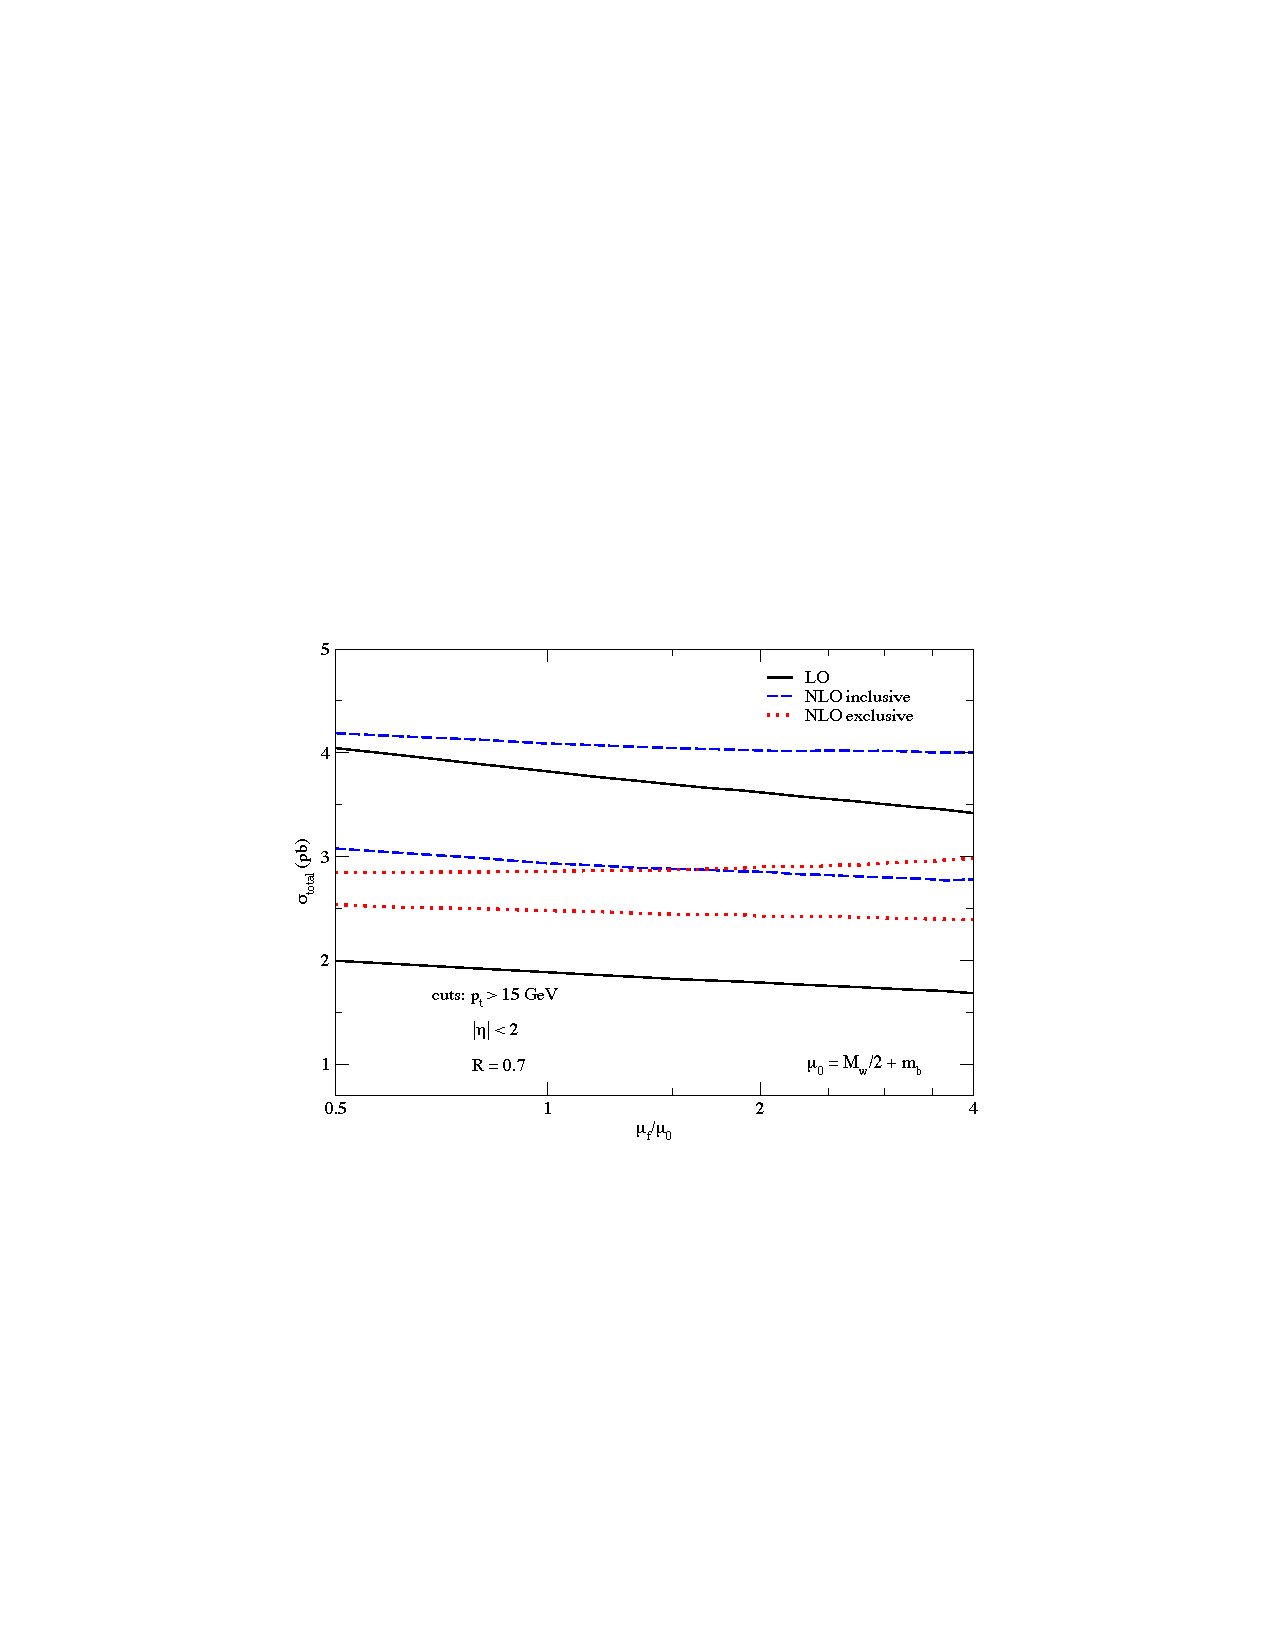
\includegraphics{Figures/2006_scale.pdf}
		%\rule{35em}{0.5pt}
	\caption[Wbb NLO scale dependence]{Wbb NLO scale dependence\cite{FebresCordero:2006sj}}
	\label{fig:2006_scale}
\end{figure}
\par New results published in 2007 explored in particular NLO corrections for events with W boson and two jets where at least one is b-tagged. It was shown that for LHC the correction factor is $\approx 1.9$. This paper was interesting in particular for it's study of soft and collinear topologies, where two b quarks merge into one. Additionally, b quark in the initial state was considered giving rise to the processes like $bq\rightarrow Wbq'$ shown in figure \ref{fig:5FS_diag}. Parton distribution function for b quark needed to be determined perturbatively using DGLAP equations. Other approach is to consider a gluon in the initial state which then splits to $b\bar{b}$. 
\begin{figure}[htbp]
	\centering
		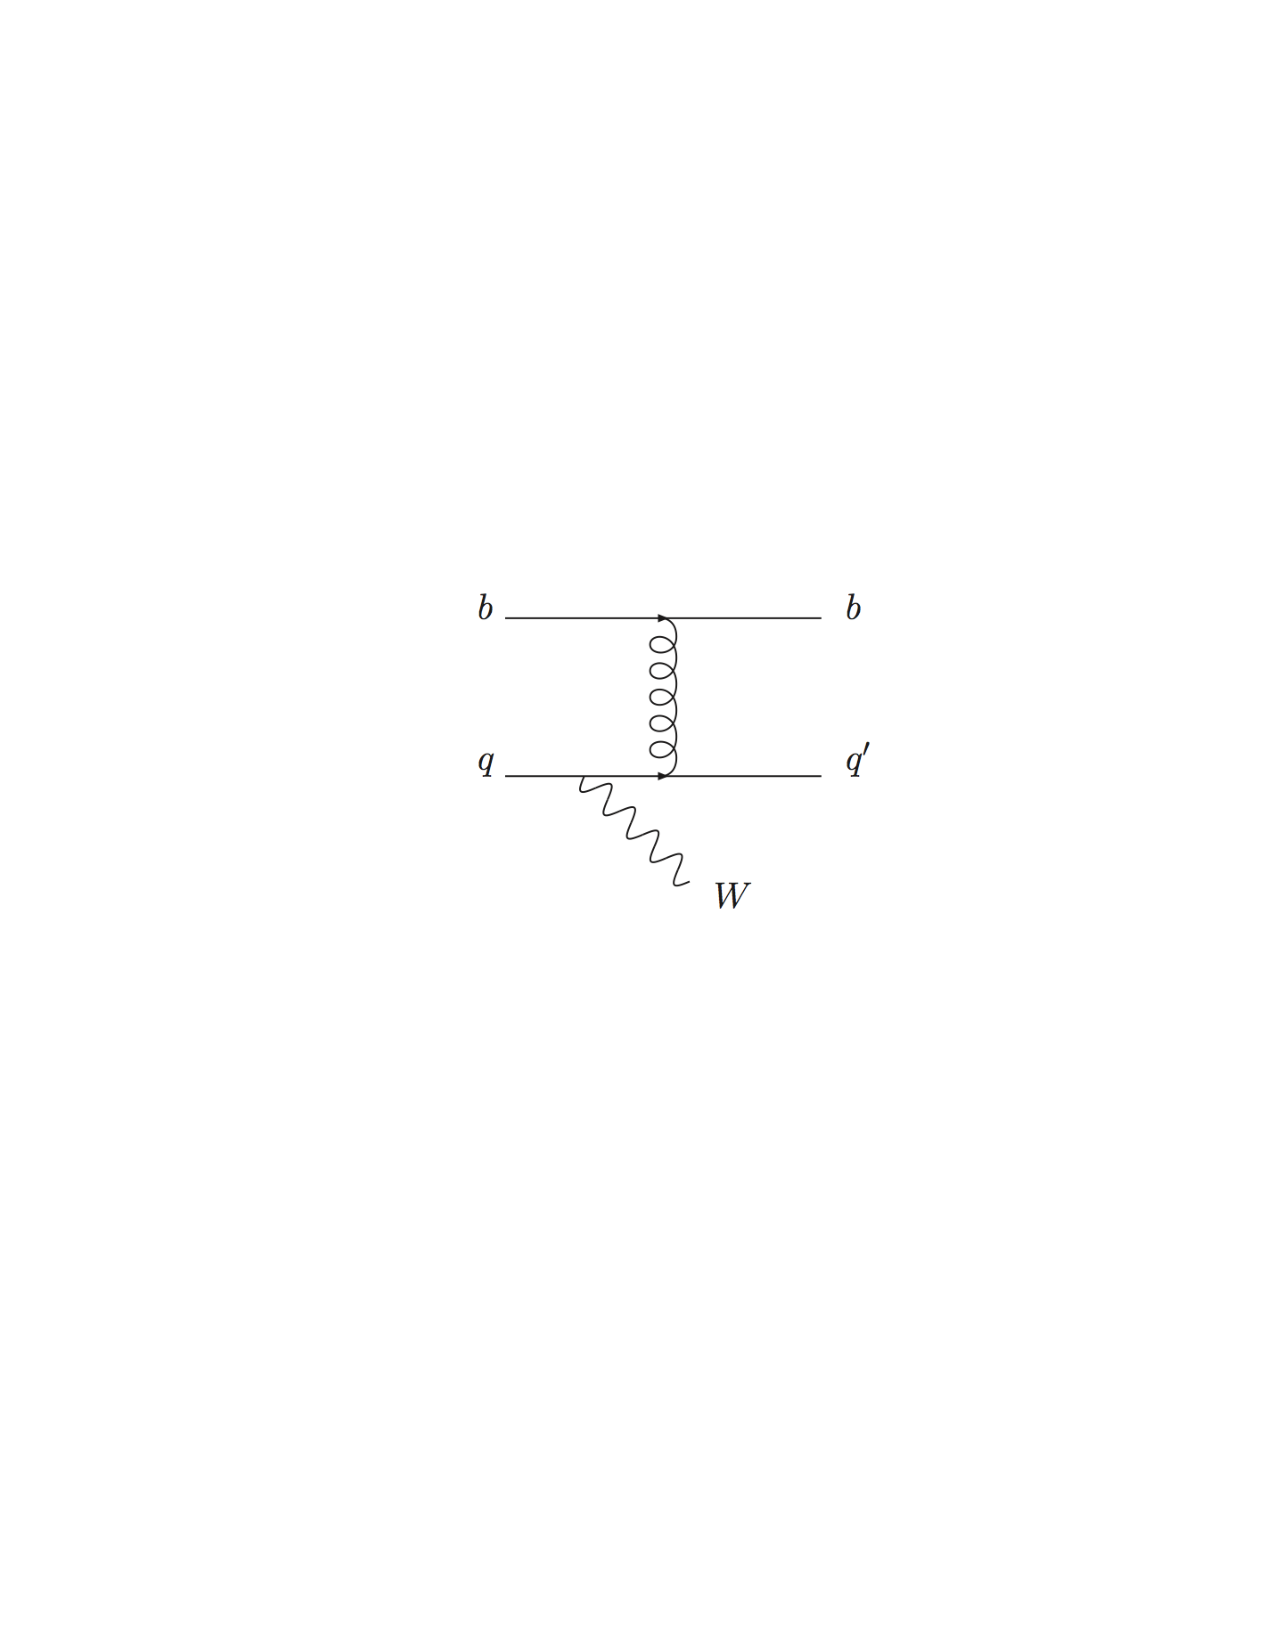
\includegraphics{Figures/5FS_diag.pdf}
		%\rule{35em}{0.5pt}
	\caption[Wbb production within 5 flavor scheme]{Wbb production within 5 flavor scheme}
	\label{fig:5FS_diag}
\end{figure}

\subsubsection{Double parton scattering}
\label{sec:DPS}
\cite{Quackenbush:2011bf}
\cite{Gaunt:2009re}
\par Multiple parton interactions happen due to composite nature of the proton. Usually inside a proton, only one parton has significant fraction of proton momentum $x$ to produce a hard scattering. However, sometimes can happen that two such partons exist which results in two hard scatterings in the same collisions. This phenomenon is called Double Parton Scattering (DPS). In the framework of this thesis, this means that two partons are responsible for creation of a W boson and other two for creation of pair of b jets. 
\par Double parton scattering cannot be modeled in the framework of preturbative QCD, but it is approximated using simulations. The phenomenology of DPS starts from the assumption that factorization between two hard processes is possible, as well as factorization between hard processes and proton kinematics. Cross sections for hard scatterings are computed separately of each pair of partons. However, instead of using regular parton distribution functions, a new set of distribution functions has been defined which are called Double Parton Distribution Functions (dPDFs). Factorized cross section for two hard processes A and B to happen in proton-proton scattering can be written as:
\begin{equation}
\begin{split}
\sigma_{(A,B)}^{DPS} \approx \sum\limits_{i,j,k,l} \int & dx_1 dx_2  dx'_1 dx'_2 d^2b  \Gamma_{ij}(x_1,x_2,b;Q_1,Q_2)\sigma_{ik}^A(x_1,x'_1) \\
 & \sigma_{jl}^B(x_2,x'_2) \Gamma_{kl}(x'_1,x'_2,b;Q_1,Q_2)
\end{split}
\end{equation}
\par Parton level cross sections are denoted with $\sigma_{ik}$, for hard process between partons $i$ and $k$, and $\sigma_{jl}$ for hard process between partons $j$ and $l$. These are the same as for single parton scattering and are know for most of the processes of interest today. Quantity $\Gamma_{ij}(x_1,x_2,b;t_1,t_2)$ represents double parton distribution function which describes the probability of finding a parton $i$ with momentum fraction $x_1$ at scale $Q_1$ inside a proton together with a parton $j$ with momentum fraction $x_2$ at scale $Q_2$. Another parameter in this distribution function is $b$ which describes transverse distance between two partons. Scales $Q_1$ and $Q_2$ and correspond to characteristic scales of hard processes $A$ and $B$. For example in the framework of this thesis W boson production would correspond to process $A$ and production of two b jets would correspond to process $B$.  

\begin{figure}[htbp]
	\centering
		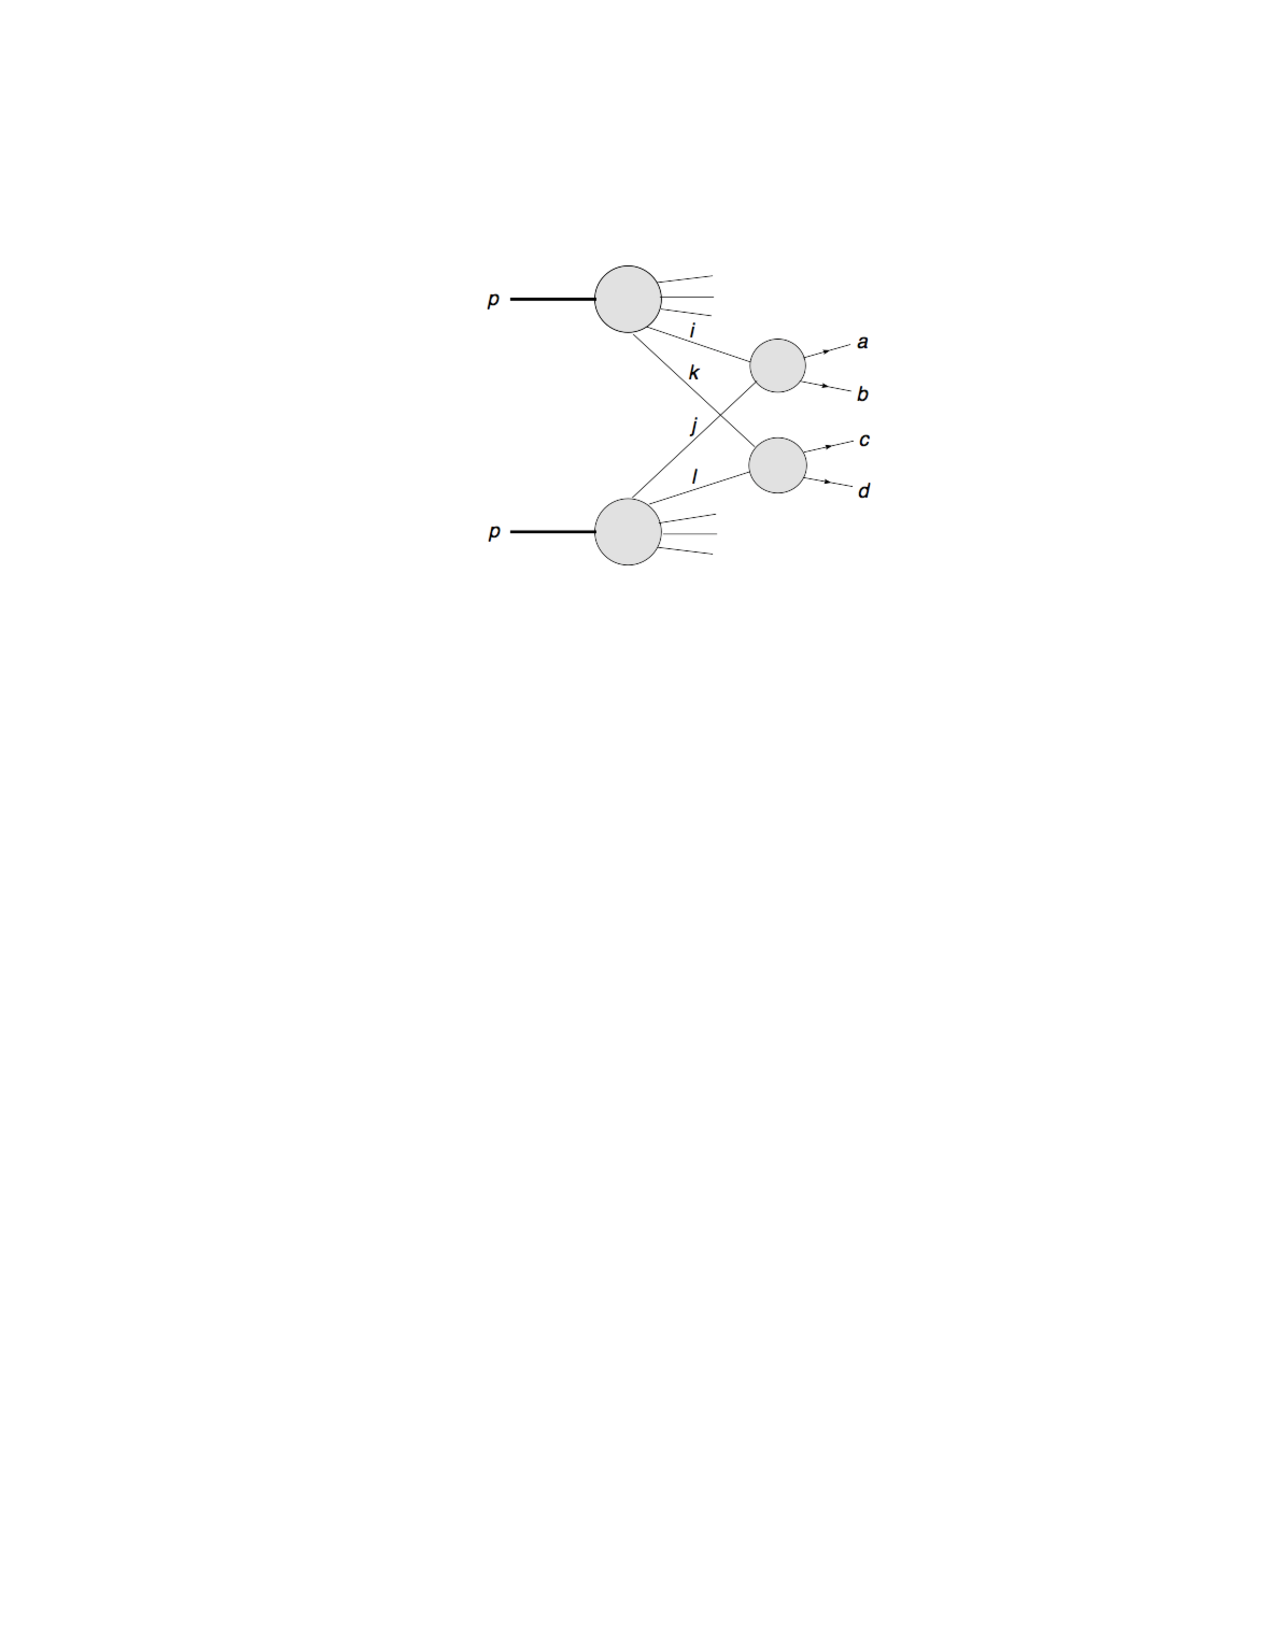
\includegraphics{Figures/DPS_diag.pdf}
		%\rule{35em}{0.5pt}
	\caption[Double parton scattering]{Double parton scattering}
	\label{fig:DPS_diag}
\end{figure}



%----------------------------------------------------------------------------------------
%	SECTION 2.3
%----------------------------------------------------------------------------------------

\section{Previous measurements}
\label{sec:2.3}
	\par Previous measurements of a W boson produced in association with b quarks have been performed on different experiments. However, the final states and phase space used in these measurements were different, which means that the results cannot be directly compared, but they can be compared with theoretical predictions. This process was measured for the first time at Tevatron with D0 and CDF experiments at $\sqrt{s} =$ 1.96 TeV. The CDF collaboration published its result in 2009 and the cross-section measured is that of “jets from b-quarks produced with a W boson”\citep{Aaltonen:2009qi}. The event selection is based on reconstructing a leptonically decaying W boson, and one or two jets where at least one has to be b-tagged. Events with jets from light quarks are vetoed with a cut on the secondary vertex mass. Contribution of other background events containing a b quark in final state (e.g. events with top quark) is estimated using Monte Carlo simulations. The measured cross section is 2.8 standard deviations higher than corresponding theoretical prediction. \\
	D0 collaboration published their result in 2012. with somewhat different phase space definition\citep{D0:2012qt}. The difference with respect to the CDF measurement consists in the inclusion of the events with 3 jets and reduced pseudorapidity range in which the measurement was performed. The measurement technique is similar to that of CDF, although b-tagging algorithms were slightly different. The measured cross section was in good agreement with the Standard model prediction.\\
	First measurements at the LHC were published by the ATLAS collaboration based on 36/pb of integrated luminosity at $\sqrt{s} =$ 7 TeV. One year later they improved their measurement using $4.6/$fb \cite{Aad:2013vka}. Selected events contain one reconstructed electron or muon, significant amount of missing transverse energy and one or two jets where exactly one is b-tagged. The phase space is divided in two regions, depending on the number of jets. Events with exactly 2 b jets and events with more than 2 jets are vetoed in order to suppress background events from top quark decay. The results are shown in Figure \ref{fig:atlas_tot}. The cross section measurement in the one jet region shows an excess corresponding to 1.5 standard deviations. In the two jet region, the measured cross section is in good agreement with theoretical predictions. A differential cross section measurement as a function of leading b jet transverse momentum has been performed for the first time and shown in figure \ref{fig:atlas_diff}. The cross section measurement in the one jet region is again higher that NLO predictions but within theoretical and experimental uncertainties. The cross section measured for the events with two jets is in good agreement with the theoretical prediction.
\begin{figure}[htbp]
	\centering
		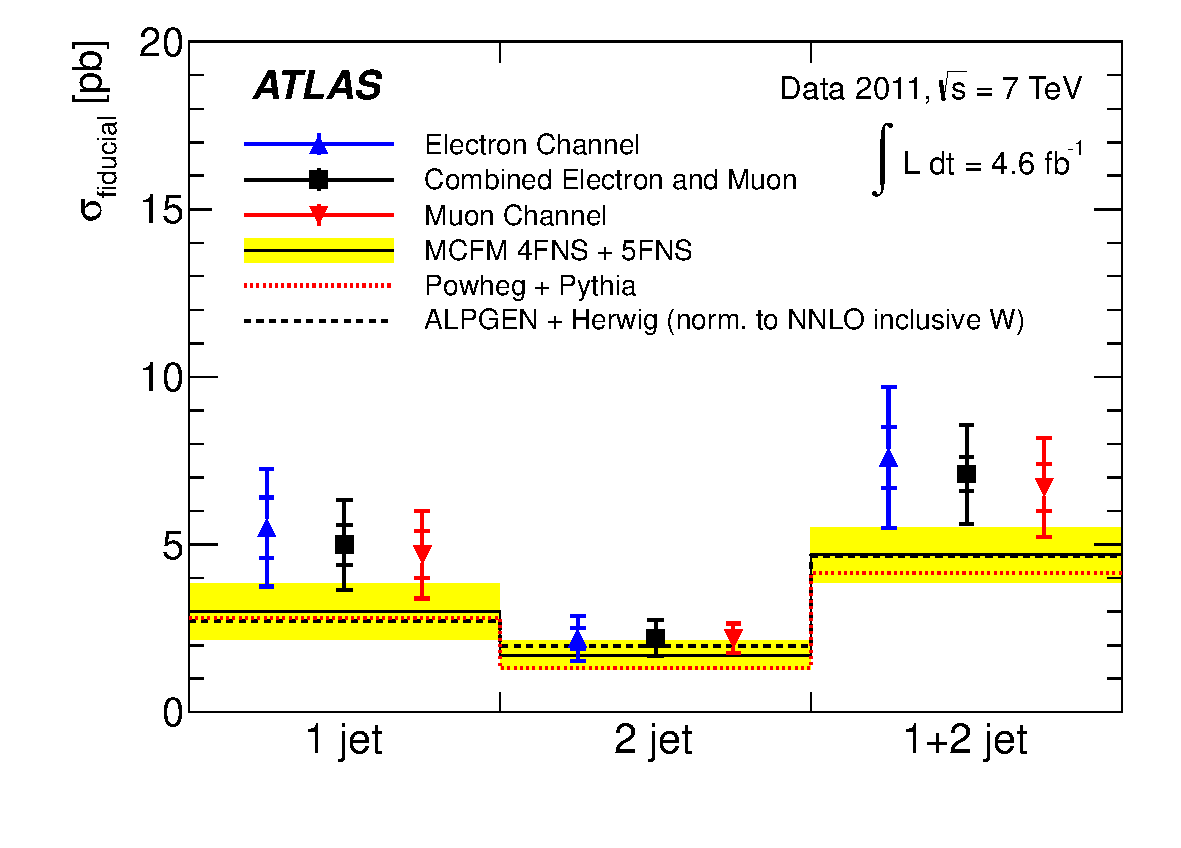
\includegraphics[width=0.7\linewidth]{Figures/atlas_total.pdf}
		%\rule{35em}{0.5pt}
	\caption[Atlas Wbb total cross section measurement]{Measured fiducial cross-sections in the electron, muon, and combined electron and muon channels. The cross-sections are given in the 1-jet, 2-jet, and 1+2-jet fiducial regions.\cite{Aad:2013vka} }
	\label{fig:atlas_tot}
\end{figure}
\begin{figure}
\centering
  \begin{subfigure}{.5\textwidth}
  	\centering
  	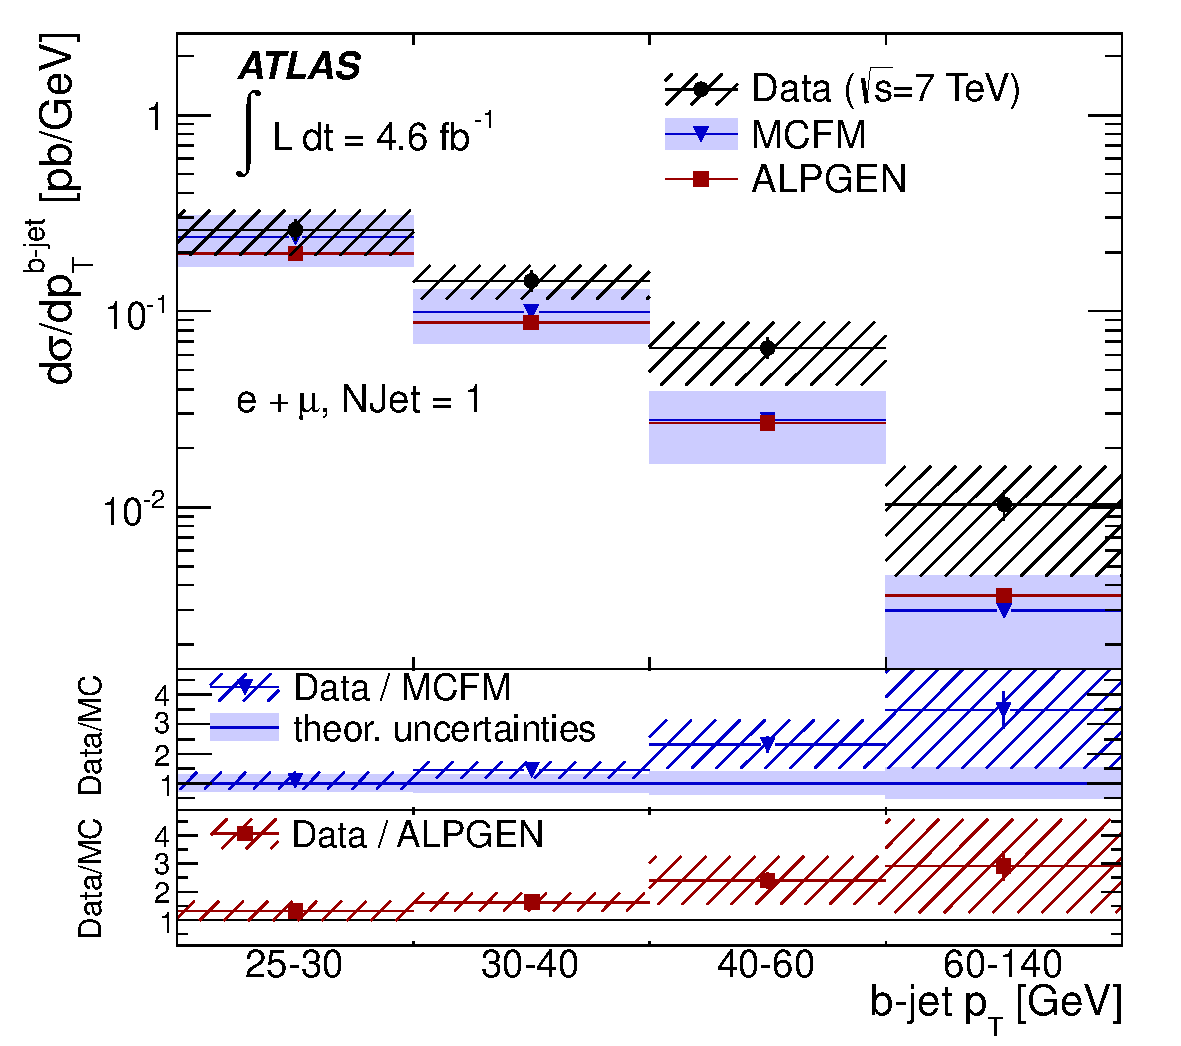
\includegraphics[width=\linewidth]{Figures/atlas_diff1j.pdf}
	\caption{}  
  	\label{fig:atlas_diff1j}
\end{subfigure}%
\begin{subfigure}{.5\textwidth}
  \centering
  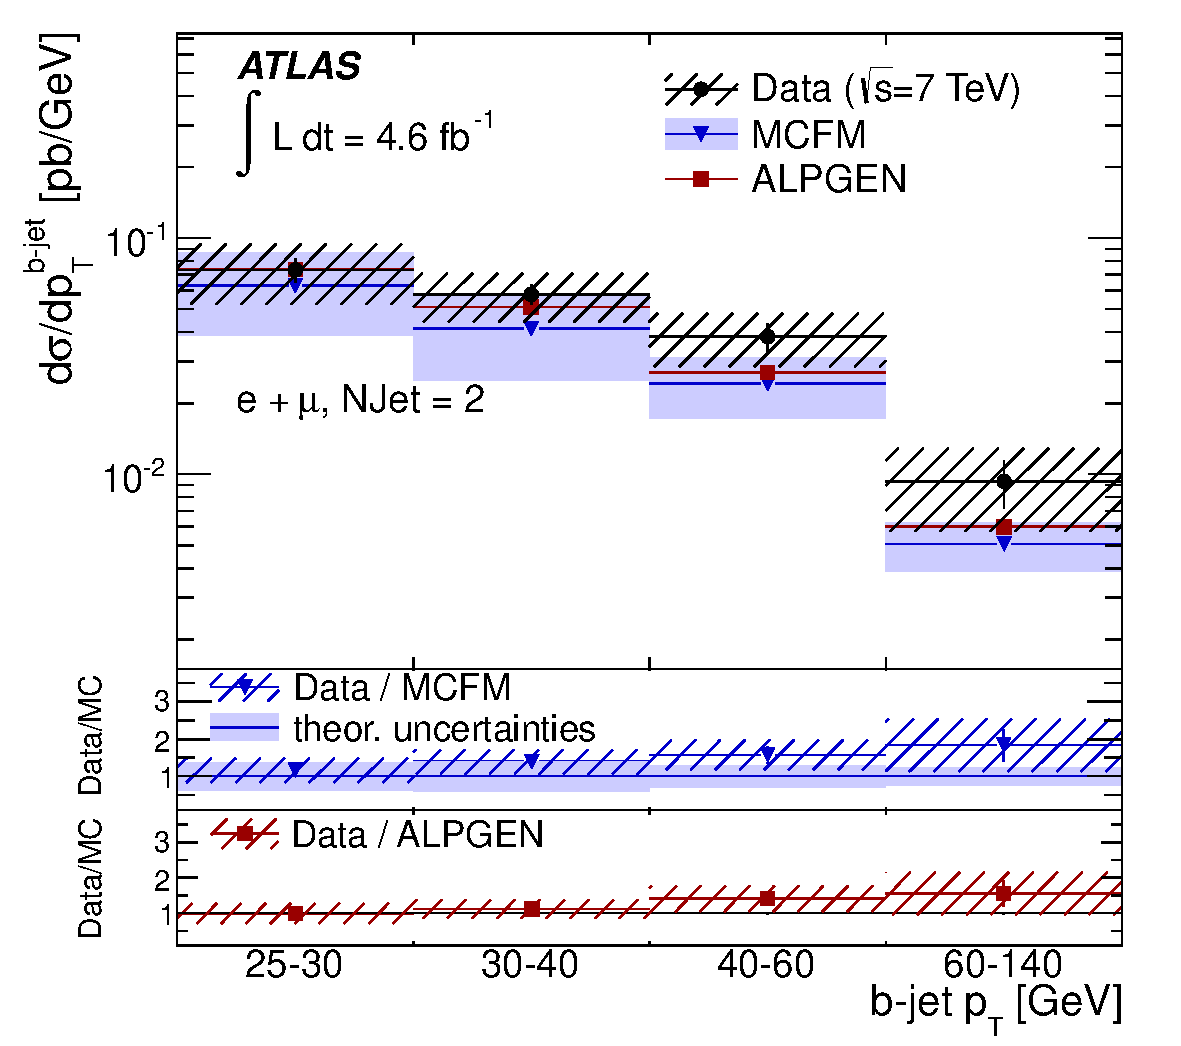
\includegraphics[width=\linewidth]{Figures/atlas_diff.pdf}
  \caption{}
  \label{fig:atlas_diff2j}
\end{subfigure}
\caption[Measured differential W+b-jets cross-sections as a function of leading b-jet $p_{T}$]{Measured differential W+b-jets cross-sections as a function of leading b-jet $p_{T}$ in the 1-jet (\ref{fig:atlas_diff1j}) and 2-jet (\ref{fig:atlas_diff2j}) fiducial regions, obtained by combining the muon and electron channel results. \cite{Aad:2013vka}}
\label{fig:atlas_diff}
\end{figure}		
The CMS collaboration published its results corresponding to data collected during 2011. The measured events contained a muon and missing transverse energy in the final state, together with two b-tagged jets. The measured cross section is in excellent agreement with the Standard model prediction.\citep{Chatrchyan:2013uza}

\begin{figure}[htbp]
	\centering
		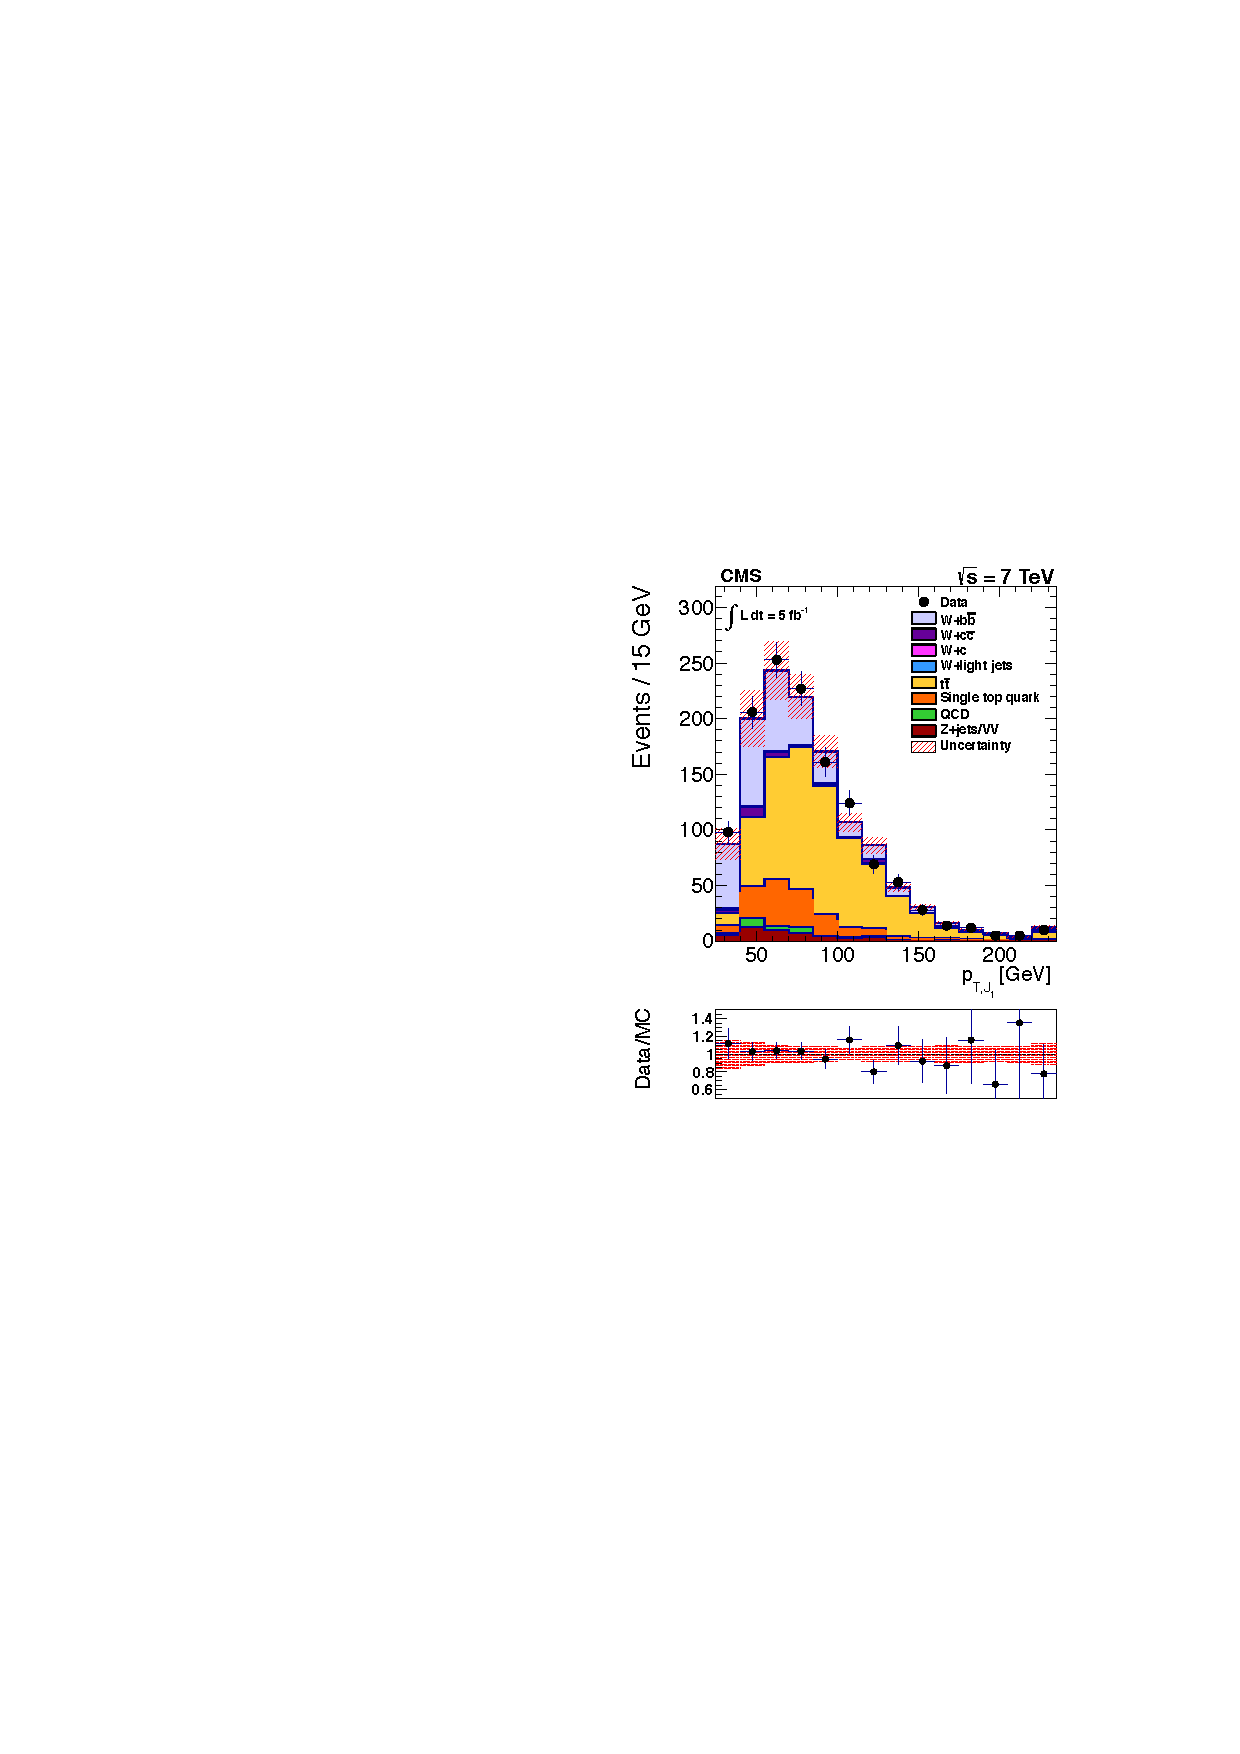
\includegraphics{Figures/cms_tot.pdf}
		%\rule{35em}{0.5pt}
	\caption[CMS Wbb total cross section measurement]{CMS Wbb total cross section measurement\cite{Chatrchyan:2013uza} }
	\label{fig:cms_total}
\end{figure}